% !TeX root = ../pyfracpaq-user-manual.tex
\major{Preparar o ambiente e iniciar}\label{sec:inicio}
Obtenha a pasta do código pelo GitHub, por clone ou download ZIP. Abra a pasta que contém \code{run_gui.py} e \code{requirements.txt}. O uso normal exige Python 3.13 e as bibliotecas; não é necessário instalar o pacote PyFracPaQ.

\subsection{Python e ambiente virtual}
No macOS, com Python 3.13 disponível, execute na raiz:
\begin{verbatim}
python3.13 -m venv .venv
.venv/bin/python -m pip install -r requirements.txt
.venv/bin/python -m pip check
.venv/bin/python run_gui.py
\end{verbatim}
Uma alternativa, na mesma pasta, é \code{.venv/bin/python -m pyfracpaq}. A instalação inicial das bibliotecas pode exigir internet. Depois, as análises funcionam localmente. Não altere silenciosamente as versões fixadas em requirements.txt.

\subsection{Miniforge e VS Code}
Com Miniforge, prepare um ambiente separado:
\begin{verbatim}
conda create -n pyfracpaq python=3.13 pip
conda activate pyfracpaq
python -m pip install -r requirements.txt
python -m pip check
python run_gui.py
\end{verbatim}
No VS Code, abra a pasta e use \control{Python: Select Interpreter}. Selecione o Python da \code{.venv} ou do ambiente Miniforge. Execute \code{run_gui.py} ou uma das configurações de Run and Debug. A extensão Python atende à seleção/execução; Python Debugger é necessária às configurações de depuração.

Foram verificados CPython 3.13.18 e Miniforge/Python 3.13.13 no macOS arm64. Windows/Linux ficam para testes posteriores do mantenedor; não se declara certificação dessas plataformas. Um ambiente chamado pyfracpaq pode já existir com outra versão: confira \code{python --version} antes de instalar.

\subsection{O que é necessário na pasta}
O programa usa \code{pyfracpaq/}, seus recursos, o launcher e as bibliotecas. \code{examples/} e este manual ajudam no uso. Testes, relatórios de auditoria e scripts internos são material de desenvolvimento do clone completo; não são necessários para executar. O ZIP de uso os exclui. Não é necessário manter a distribuição MATLAB na pasta.

\subsection{Diretório de trabalho e arquivos existentes}
A saída normal é o diretório corrente de execução. Ao iniciar pela raiz, os resultados ficam nessa raiz; para trabalhos separados, use uma cópia de trabalho ou inicie com o caminho absoluto de \code{run_gui.py} a partir da pasta de saída, usando o mesmo Python preparado. O modo por módulo, sem instalar o projeto, deve ser iniciado na raiz.

A mesma tag reutiliza os mesmos nomes e substitui arquivos anteriores. Alguns intermediários têm nomes fixos e não recebem tag. Preserve as entradas originais e separe trabalhos antes de clicar Run. A conversão SVG é uma exceção de destino: seus TXT ficam ao lado do SVG.

\major{Dados, geometria, escala e orientação}\label{sec:dados}
\subsection{Traço, segmento e nó}
Um \emph{traço} é a polilinha de uma fratura mapeada. Seus vértices são nós de entrada; dois nós consecutivos formam um segmento. Esses nós geométricos não são automaticamente os nós topológicos I/Y/X, calculados depois.

Para \(\mathbf p_i=(x_i,y_i)\),
\begin{equation}
\ell_i=\|\mathbf p_{i+1}-\mathbf p_i\|_2,
\qquad L=\sum_i\ell_i.
\end{equation}
O comprimento total \(L\) é o percurso, não a distância reta entre as pontas. O centro de um traço é interpolado a metade do percurso; o centro de um segmento é a média de suas duas pontas. Essas posições entram nos perfis e no variograma.

A área de amostragem usual é o retângulo do domínio,
\begin{equation}
A=(x_{\max}-x_{\min})(y_{\max}-y_{\min}).
\end{equation}
Não confunda essa área com a soma das áreas de blocos. Em imagens, algumas análises usam o domínio completo da imagem e os tensores usam o envelope dos nós extraídos; a área pertinente é explicitada na seção de cada família.

\subsection{Arquivo TXT de nós}
Há um traço por linha e pares X/Y separados por TAB, sem cabeçalho. Exemplo com dois traços:
\begin{verbatim}
0<TAB>0<TAB>4<TAB>0
1<TAB>2<TAB>4<TAB>2<TAB>4<TAB>6
\end{verbatim}
Substitua \code{<TAB>} por um tabulador real. O primeiro traço contém um segmento; o segundo, dois. Cada linha precisa de pelo menos dois nós distintos. Valores vazios, não finitos ou pares incompletos são recusados com localização do erro, sem leitura parcial. Duplicatas consecutivas são removidas com diagnóstico; um traço que se torna degenerado é recusado.

\subsection{Escala física}
Em \control{Scaling (pixels/metre)}, informe \(s>0\) para uma calibração conhecida. Sem escala, a unidade é pixel. O código reconstrói a geometria a partir da entrada:
\begin{equation}
 x_m=x_{px}/s,\quad y_m=y_{px}/s,\quad
 L_m=L_{px}/s,\quad A_m=A_{px}/s^2.
\end{equation}
Não basta mudar o rótulo. Uma nova escala exige nova prévia e limpa a linha de Graphs. Intensidade tem unidade de comprimento inverso, densidade de área inversa e permeabilidade de área. A abertura digitada em Fluid flow precisa estar na unidade corrente; seu número não é convertido automaticamente quando a escala muda.

\subsection{Flips, norte e ângulos}
O ângulo bruto de um segmento é medido em relação ao eixo Y, como uma direção axial, normalmente representada em \([0,180]\). Uma expressão geométrica equivalente é
\(\beta=\operatorname{atan2}(\Delta x,\Delta y)\), com a representação axial do programa. Norte, arredondamentos e flips são aplicados pelas rotinas específicas; não alteram os nós armazenados.

\control{Flip X-axis} e \control{Flip Y-axis} refletem a apresentação e influenciam as correções angulares das famílias pertinentes. \control{Rotate Y-axis from N (°)}, disponível nas abas que o utilizam, corrige o referencial angular. Perfis de ângulo em Graphs e o TXT bruto de ângulos/comprimentos não recebem a mesma transformação do EZROSE. Wavelets trabalha em seu raster e não aplica a correção de norte.

\begin{note}{Evitar duas correções da mesma geometria}
Não redesenhe os nós para compensar um flip que já será aplicado na interface. Confira a direção conhecida de uma fratura antes de interpretar rosas, tensores ou tensões. As diferenças entre os arquivos angulares são intencionais, não sinônimo de erro de unidade.
\end{note}

\subsection{SVG: conjuntos por cor}
Aceitam-se \code{line}, \code{polyline} e caminhos absolutos M/L, com stroke hexadecimal por atributo, estilo inline ou grupo. O exemplo \code{examples/colours.svg} contém duas cores. Curvas, transformações, polígonos SVG e CSS externo/classes não são convertidos silenciosamente: prepare o arquivo no editor externo.

Preview converte os nós em TXT junto ao SVG, agrupando por cor. Os nomes incluem \code{_colourHHHHHH_converted.txt}; um conjunto simples usa \code{_converted.txt}. É possível recarregar um TXT de cor para análise individual. Quando pertinente, um SVG multicolorido acrescenta a figura multicolorida; cor é procedência do conjunto, não uma classe estatística inferida.
\plotfig{tracemap_multicolour.png}{Exemplo auxiliar SVG, distinto de SD11A: preservação dos grupos de cor em mapa de traços.}{fig:svg}

\subsection{Imagens: transformada de Hough}\label{sec:hough}
Escolha JPEG/TIFF grayscale de oito bits, quadro único. RGB, alpha, imagens indexadas e maior profundidade não são convertidos automaticamente pela GUI. Use o utilitário de pré-processamento quando necessário e confira seu resultado visualmente.

O complemento identifica pixels diferentes de branco, remove pixels isolados e calcula a Hough padrão:
\begin{equation}
\rho=x\cos\theta+y\sin\theta.
\end{equation}
Uma linha de pixels acumula votos no espaço \((\theta,\rho)\). O programa usa passo angular de \(0{,}5^\circ\), passo de \(\rho\) de um pixel e coordenadas finais de imagem em base 1. Isso detecta segmentos retos: não substitui uma digitalização interpretativa de fraturas curvas.

\begin{tabularx}{\linewidth}{@{}p{.35\linewidth}X@{}}
\toprule Controle & Efeito no Preview de imagem\\\midrule
\control{Number of Hough peaks} & Limite de picos: inteiro de 100 a 5000; mais picos podem incluir ruído.\\
\control{Hough threshold} & Fração do máximo do acumulador: \(0<t\leq1\). Menor limiar inclui picos mais fracos.\\
\control{Merge gaps less than} & FillGap: distância em pixels usada para unir trechos compatíveis; maior que 1.\\
\control{Discard lengths less than} & MinLength: comprimento mínimo em pixels; maior que 1.\\\bottomrule
\end{tabularx}
Os defaults são 1000, 0.33, 5 e 3. Alterá-los exige nova prévia. A figura diagnóstica é exportada no Preview, antes do Run. Se nenhuma linha for encontrada, o diagnóstico permanece disponível, mas não há rede para analisar. O exemplo \code{examples/network.tif} é apropriado para testar esse fluxo.
\plotfig{Houghstuff.png}{Diagnóstico Hough do exemplo auxiliar de imagem. Os parâmetros são os defaults; não é uma rasterização do SD11A.}{fig:hough}

\major{Primeiro roteiro com SD11A}\label{sec:roteiro}
\subsection{Carregar e conferir a prévia}
\begin{enumerate}
\item Abra o programa e mantenha \control{Node file}.
\item Use Browse ou informe o caminho de \code{examples/SD11A.txt}.
\item Deixe a escala vazia, sem flips, e clique \control{Preview}.
\item Confira os números da tabela abaixo. As seis abas ficam disponíveis depois de uma prévia válida.
\item Troque \control{Filename tag for this run} para \code{SD11A}; escolha as saídas e clique \control{Run}.
\end{enumerate}
\begin{center}\begin{tabular}{@{}lr@{}}\toprule
Grandeza & Valor de referência\\\midrule
Traços / segmentos / nós & 445 / 1076 / 1521\\
\(x_{\min},x_{\max}\) & 0 ; 1997.7\\
\(y_{\min},y_{\max}\) & 1.8 ; 1988.5\\
Área do envelope & 3968830.59 pixels\(^{2}\)\\\bottomrule
\end{tabular}\end{center}
\begin{figure}[htbp]\centering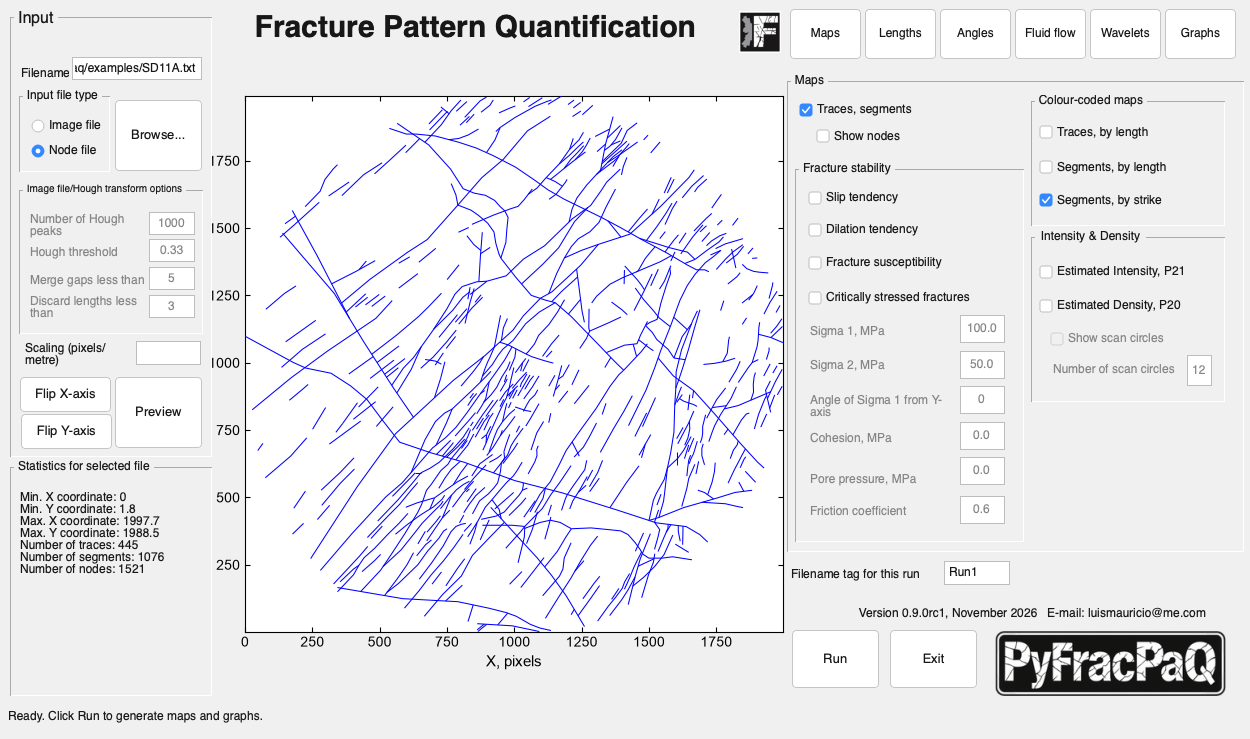
\includegraphics[width=\linewidth]{ui-preview.png}\caption{Prévia real de SD11A e estatísticas. A captura conserva a tag default Run1; use SD11A no roteiro para distinguir seus arquivos.}\label{fig:preview}\end{figure}

\Needspace{14\baselineskip}
\subsection{Parâmetros das figuras deste manual}\label{sec:parametros}
As ilustrações analíticas reutilizam uma execução revisada do SD11A com estes parâmetros, que \emph{não são todos os defaults da GUI}:
\begin{longtable}{@{}p{.43\linewidth}p{.49\linewidth}@{}}
\toprule Grupo & Configuração ilustrada\\\midrule\endhead
Entrada & Sem escala física, sem flips, norte \(0^\circ\), tag SD11A.\\
Comprimentos & 20 intervalos solicitados; censura desligada; cortes MLE Lower=0 e Upper=0.\\
Ângulos & 20 intervalos solicitados no histograma; rosa de \(10^\circ\), sem ponderação por comprimento; cor/média ativadas.\\
Maps circular & 12 círculos no lado menor; Show scan circles ativado.\\
Conectividade & 12 blocos; tolerância I\(\to\)Y de 2.0 pixels.\\
Tensões & \(\sigma_1=100\), \(\sigma_2=50\) MPa; azimute \(0^\circ\), coesão=0, pressão de poros=0, atrito=0.6. Valores ilustrativos.\\
Permeabilidade & Abertura fixa 0.001 pixel, \(\lambda=1\); exemplo sem calibração física.\\
Wavelets & Morlet, a=32, L=2, incremento \(90^\circ\). É uma grade curta de demonstração.\\
Graphs & Linha horizontal de \((0,995.15)\) a \((1997.7,995.15)\), 12 círculos.\\\bottomrule
\end{longtable}
Graphs recebe pontos por cliques, não por campos de coordenadas. A linha exata das figuras foi definida no roteiro de comparação; uma seleção manual aproximada pode mudar as interseções. MLE usa uma seed registrada na execução ilustrada; a GUI gera seeds próprias, portanto avaliações Monte Carlo podem variar.

\subsection{Estados, progresso e revisão das saídas}
Editar entrada, escala, tipo ou parâmetros Hough invalida a prévia. Run fica desabilitado enquanto não houver geometria válida ou enquanto houver operação em andamento. Apenas parâmetros necessários às análises selecionadas são validados. Uma mensagem inválida identifica o campo/aba para correção; seleções em outras abas permanecem disponíveis.

O cálculo ocorre em segundo plano; a apresentação/exportação das figuras é sequenciada na interface. Aguarde a conclusão: MLE e Wavelets podem demorar. A janela principal não possui um botão Cancel geral; Exit solicita encerramento em uma etapa segura. As figuras são janelas independentes com a barra de ferramentas Matplotlib para navegação; fechá-las não altera os dados.
